\documentclass[9pt,a4paper,twoside]{rho}
\usepackage[polish]{babel}
\usepackage{rhoenvs}
\usepackage{booktabs}

%----------------------------------------------------------
% TITLE
%----------------------------------------------------------

\title{Raport zaliczeniowy\\
Przewidywanie zużycia paliwa}

%----------------------------------------------------------
% AUTHOR
%----------------------------------------------------------

\author{Aliaksandr Mikulka\\
MSiD Lab Grupa 3\\
276751@student.pwr.edu.pl
}

%----------------------------------------------------------
% DATES
%----------------------------------------------------------

\dates{Raport wygenerowany \today}

\begin{document}

    \maketitle
\section*{Opis Problemu}

    Problemem wybranym do badań jest przewidywanie zużycia paliwa samochodu w zależności od innych czynników. Analiza zbioru danych może wykazać przybliżone zużycie paliwa samochodu na podstawie danych o jego silniku, paliwie które jest wykorzystane, warunkach pogodowych oraz populacji badanego obszaru. Celem projektu jest zbadanie powyższych zależności oraz stworzenie modelu który potrafi przewidzieć zużycie paliwa samochodu.

\section*{Zbiór danych i jego przetwarzanie}
    \subsection*{Zbiór danych}
    
        Dla rozwiązania powyższego problemu zostały wykorzystane cztery zbiory danych. Wszystkie te dane były zebrane na terytorium Kanady więc obszarem badanym będzie ten kraj.
        
        Pierwsze dwa zbiory były pobrane ze strony internetowej kaggle.com.
        \begin{itemize}
        \item Pierwszy zbiór \cite{kaggle_fuel} zawiera informacje o roku produkcji, marce i modelu, typu samochodu, charakterystykach silnika i transmisji oraz dane o paliwie i wskaźnikach jego zyżycia w różnych przypadkach.
        \item Drugi zbiór \cite{kaggle_temp} zawiera informacje o średnich temperaturach oraz ilości opadów w każdym miesiącu.
        \item Trzeci zbiór \cite{statcan} był pobrany ze strony www150.statcan.gc.ca . Ten zbiór zawiera informacje o ilości samochodów wyprodukowanych w każdym roku.
        \item Ostatni zbiór \cite{wiki_demographics_canada} był pobrany ze strony wikipedia.org . Zbiór jest zeskrobany z tabeli która zawiera informacje o populacji Kanady.
        \end{itemize}
    \subsection*{Przetwarzanie danych do analizy}
        Każdy zbiór jest przetwarzany w taką postać, w ktorej on będzie praktyczny do wykorzystania i przedstawiania danych.
        \begin{itemize}
            \item Dane o temperaturze (tabela \ref{tab:weather_data}) są przetwarzane do postaci, gdzie dla każdego roku są wartości reprezentujące srednią temperaturę, ogólną ilość opadów i śniegu.
            \item Zbiór o ilości sprzedanych samochodów (tabela \ref{tab:yearly_sells}) zawiera dużo zbędnej informacji. Z tego zbioru są wykorzystane tylko te dane, które reprezentują ilość sprzedanych samochodów w każdym roku.
            \item Zbiór danych reprezentujący populacje Kanady (tabela \ref{tab:average_population}) jest zeskrobany z tabeli wikipedii. Z tego zbioru potrzebujemy tylko dane o populacji w każdym roku.
            \item W zbiorze danych o samochodach, ich charakterystykach i wskaźnikach zużycia paliwa (tabela \ref{tab:vehicle_data}) niektóre dane mają takie same wartości, tylko napisane w inny sposób (np. marka napisana wielkimi lub małymi literami, typ samochodu zapisany z innym znakiem rozdielającym). Także kolumna reprezentująca typ paliwa jest przetważana do pełnej nazwy w celu łatwiejszego zrozumienia jakie paliwo jest wykorzystane.
        \end{itemize}
        
            \begin{table}[ht]
            \centering
            \caption{Dane pogodowe}
            \label{tab:weather_data}
            \begin{tabular}{cccc}
            \toprule 
            Rok & Średnia temperatura & Opady śniegu & Całkowite opady \\ 
            \midrule
            1917 & 3.397697 & 71993.4 & 282321.6 \\
            1918 & 4.601561 & 61197.0 & 299492.6 \\
            1919 & 4.422720 & 62713.9 & 294860.5 \\
            1920 & 4.473663 & 66841.0 & 299336.7 \\
            1921 & 5.045527 & 67793.2 & 323221.2 \\
            \bottomrule
            \end{tabular}
            \end{table}

            \begin{table}[ht]
            \centering
            \caption{Dane o sprzedaży samochodów}
            \label{tab:yearly_sells}
            \begin{tabular}{cc}
            \toprule
            Rok & Ilość sprzedanych samochodów \\
            \midrule
            1946 & 313373 \\
            1947 & 646494 \\
            1948 & 660518 \\
            1949 & 875066 \\
            1950 & 1315365 \\
            \bottomrule
            \end{tabular}
            \end{table}
                        

            \begin{table}[ht]
            \centering
            \caption{Coroczna Populacja}
            \label{tab:average_population}
            \begin{tabular}{cc}
            \toprule
            Rok & Populacja \\
            \midrule
            1900 & 5500000 \\
            1901 & 5600000 \\
            1902 & 5760000 \\
            1903 & 5930000 \\
            1904 & 6100000 \\
            \bottomrule
            \end{tabular}
            \end{table}

            \begin{table}[ht]
            \centering
            \caption{Dane o samochodach i zużyciu paliwa}
            \label{tab:vehicle_data}
            \begin{tabular}{cccc}
            \toprule
            Rok produkcji & Marka & Model & Typ Samochodu \\
            \midrule
            2000 & ACURA & 1.6EL & COMPACT \\	
            2000 & ACURA & 1.6EL & COMPACT \\
            2000 & ACURA & 3.2TL & MID-SIZE \\
            \midrule
            Pojemność silnika & Cylindry & Transmisja & Paliwo \\
            \midrule
            1.6 & 4 & A4 & Regular gasoline	\\
            1.6 & 4 & M5 & Regular gasoline \\
            3.2 & 6 & AS5 & Premium gasoline \\
            \midrule
            Zużycie paliwa & HWY & COMB & Emisje (mpg) \\
            \midrule
            9,2 & 6.7 & 8.1 & 186 \\
            8.5 & 6.5 & 7.6 & 175 \\
            12.2 & 7.4 & 10.0 & 230 \\
            \bottomrule
            \end{tabular}
            \end{table}
            
        Wszystkie zbiory były przeanalizowane na przedmiot brakujących danych. Tylko w zbiorze reprezentujacy średnie temperatury była znaleziona jedna zgubiona wartość o ilości opadów w 1917 roku. Ta wartość była zastąpiona przez 0 ponieważ takie stare dane nie będa potrzebne dla przewidywania.

\section*{Analiza danych i wyszukiwanie zależności}
    Następnym etapem jest wyszukiwanie zależności pomiędzy danymi które mogą pomóc w przewidywaniu zużycia. Sprzedaży samochodów będą mieć zakres od 2000 do 2022 roku.
    \subsection*{Analiza danych}

        \begin{figure}[H]
            \centering
            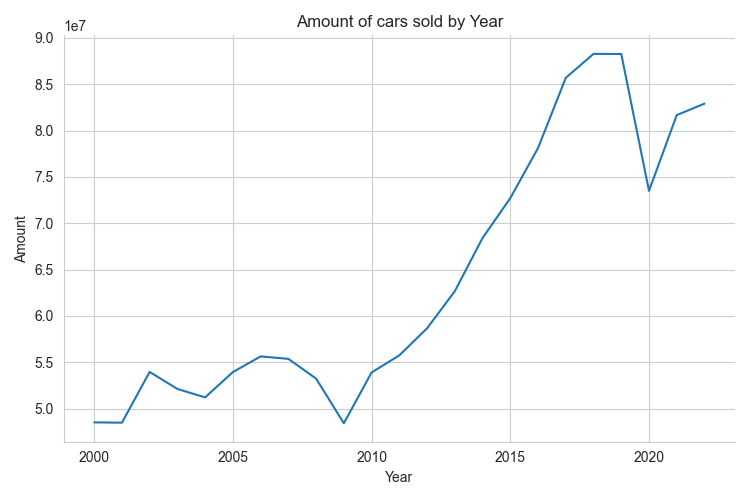
\includegraphics[width=1\columnwidth]{plots/Amount of cars sold by Year.png}
            \caption{Ilość sprzedanych samochodów według roku}
            \label{fig:amount_of_cars_sold_by_year}
        \end{figure}
    
        Dane pogodowe będą mieć zakres od 2000 do 2017 roku.
    
        \begin{figure}[H]
            \centering
            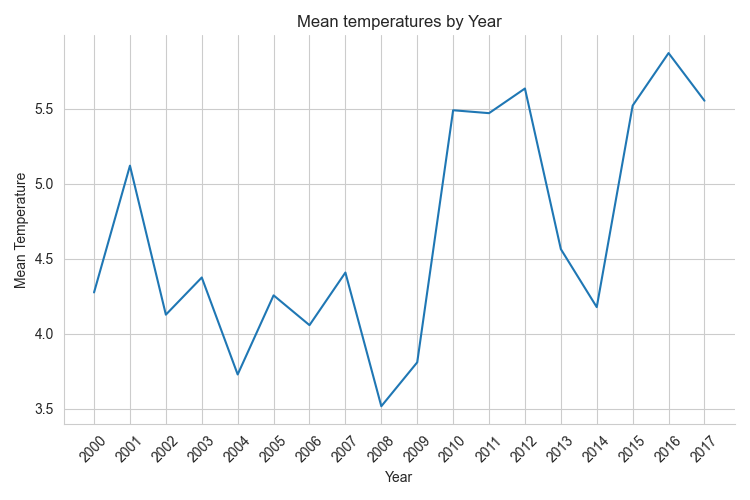
\includegraphics[width=1\columnwidth]{plots/Mean temperatures by Year.png}
            \caption{Średnie temperatury według roku}
            \label{fig:mean_temperatures_by_year}
        \end{figure}
    
        \begin{figure}[H]
            \centering
            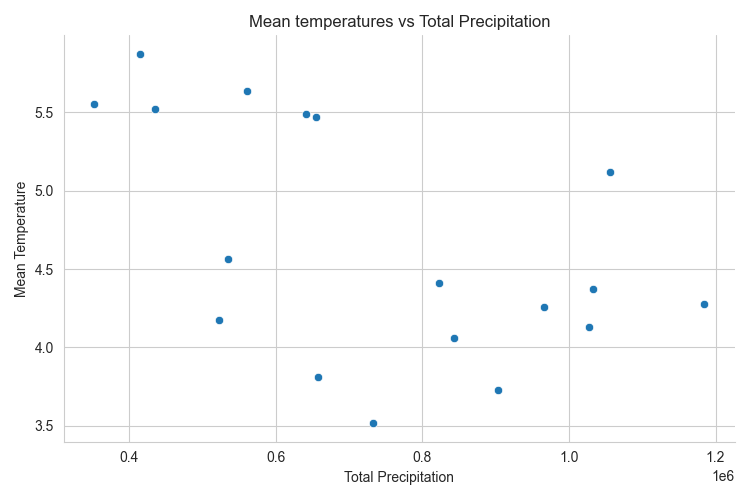
\includegraphics[width=1\columnwidth]{plots/Mean temperatures vs Total Precipitation.png}
            \caption{Zależność pomiędzy średnią temperaturą i całkowitymi opadami}
            \label{fig:mean_temperatures_vs_total_precipitation}
        \end{figure}
    
        \begin{figure}[H]
            \centering
            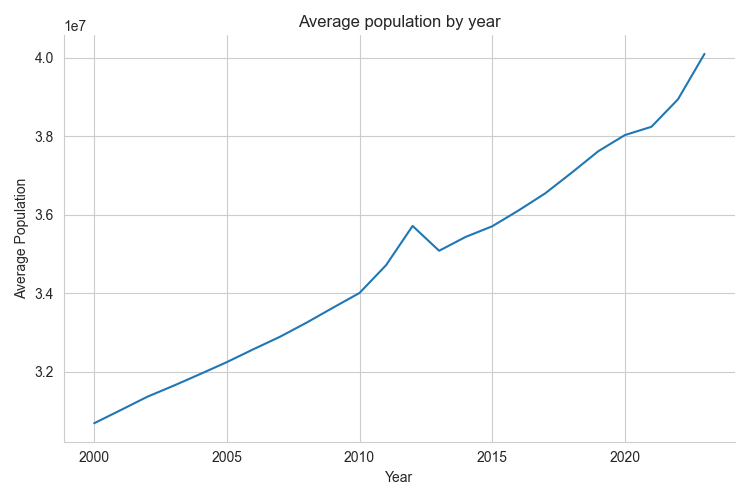
\includegraphics[width=1\columnwidth]{plots/Average population by year.png}
            \caption{Średnia populacja według roku}
            \label{fig:pop_by_year}
        \end{figure}
    
        \begin{figure}[H]
            \centering
            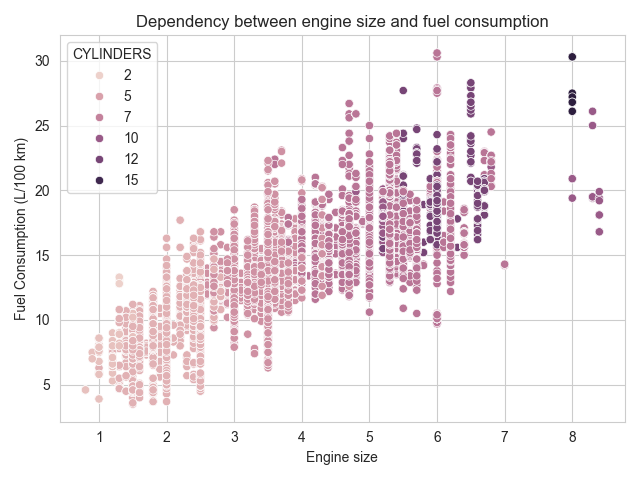
\includegraphics[width=1\columnwidth]{plots/Dependency between engine size and fuel consumption.png}
            \caption{Zależność pomiędzy pojemnością silnika i zużyciem paliwa}
            \label{fig:engine_size_vs_fuel_cons}
        \end{figure}
    
        \begin{figure}[H]
            \centering
            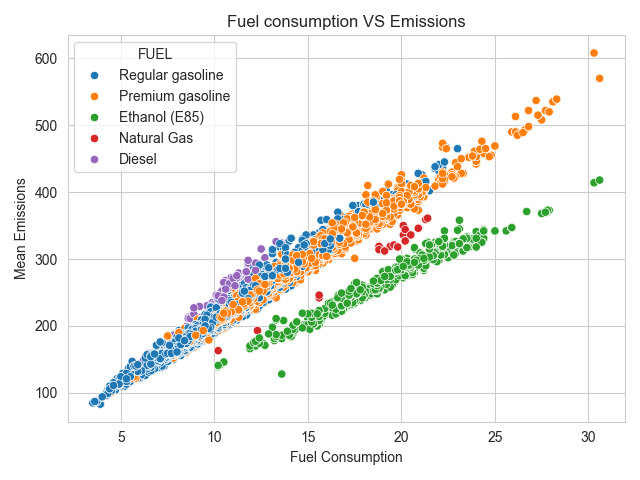
\includegraphics[width=1\columnwidth]{plots/Fuel consumption VS Emissions.png}
            \caption{Zależność pomiędzy zużyciem paliwa i emisją}
            \label{fig:fuel_cons_vs_emissions}
        \end{figure}
    
        \begin{figure}[H]
            \centering
            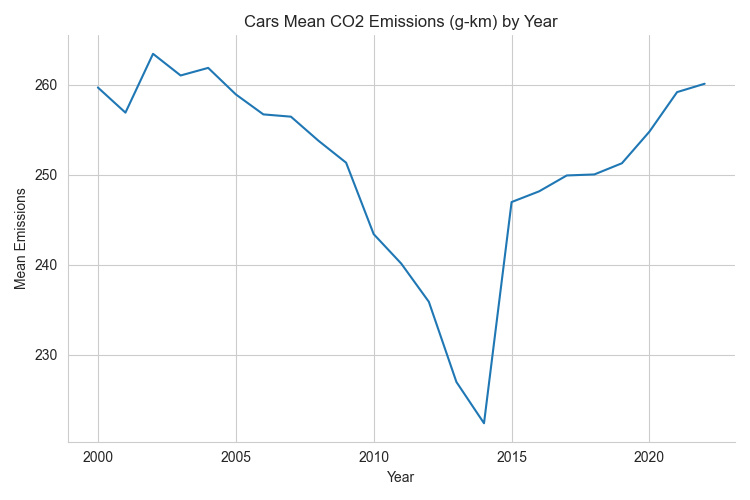
\includegraphics[width=1\columnwidth]{plots/Cars Mean CO2 Emissions (g-km) by Year.png}
            \caption{Średnia emisja samochodów według roku}
            \label{fig:cars_mean_emissions_by_year}
        \end{figure}
    
        \begin{figure}[H]
            \centering
            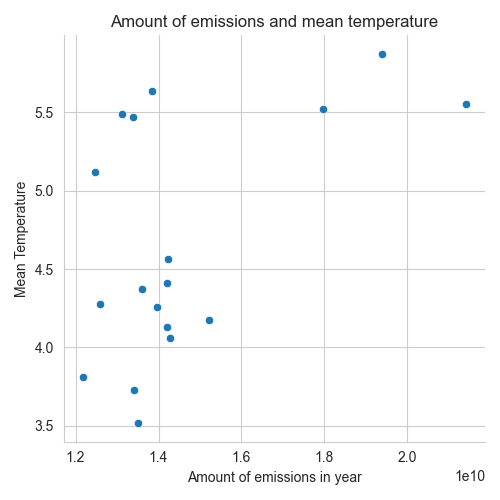
\includegraphics[width=1\columnwidth]{plots/Amount of emissions and mean temperature.png}
            \caption{Zależność między ilością emisji a średnią temperaturą}
            \label{fig:amount_emiss_vs_mean_temp}
        \end{figure}
    
        \begin{figure}[H]
            \centering
            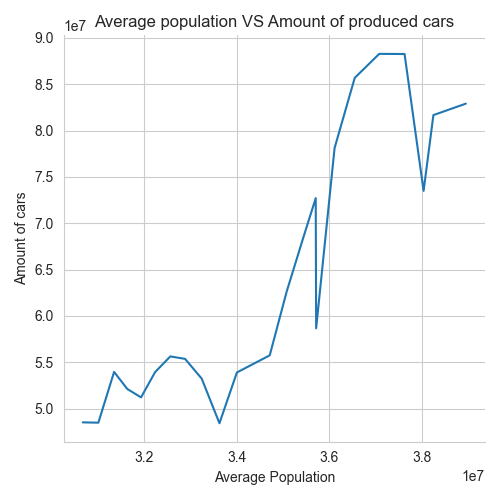
\includegraphics[width=1\columnwidth]{plots/Average population VS Amount of produced cars.png}
            \caption{Zależność liczby ludności od ilości wyprodukowanych samochodów}
            \label{fig:population_vs_produced_cars}
        \end{figure}
        
        \begin{figure}[H]
            \centering
            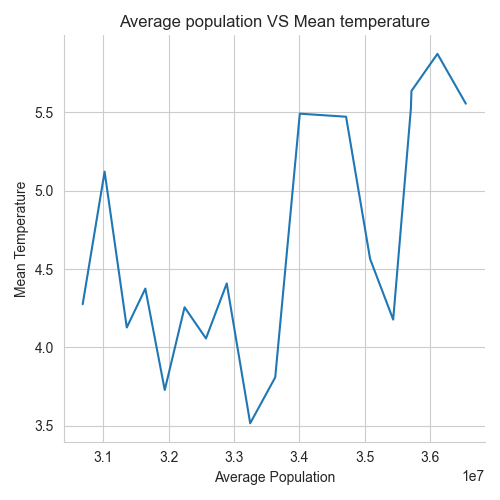
\includegraphics[width=1\columnwidth]{plots/Average population VS Mean temperature.png}
            \caption{Zależność populacji od średniej temperatury}
            \label{fig:population_vs_mean_temp}
        \end{figure}
    
        \begin{figure}[H]
            \centering
            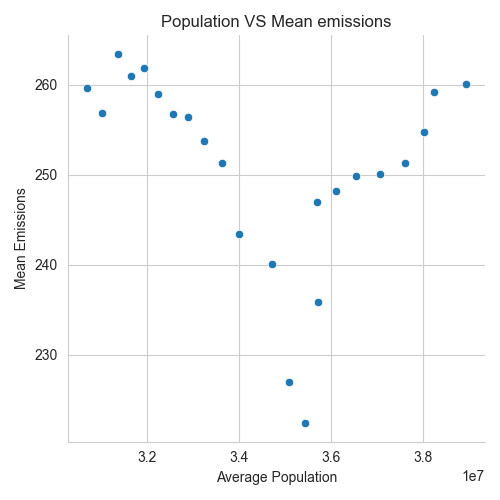
\includegraphics[width=1\columnwidth]{plots/Population VS Mean emissions.png}
            \caption{Zależność pomiędzy liczbą ludności a wielkością emisji}
            \label{fig:population_vs_emissions}
        \end{figure}
    
        \begin{figure}[H]
            \centering
            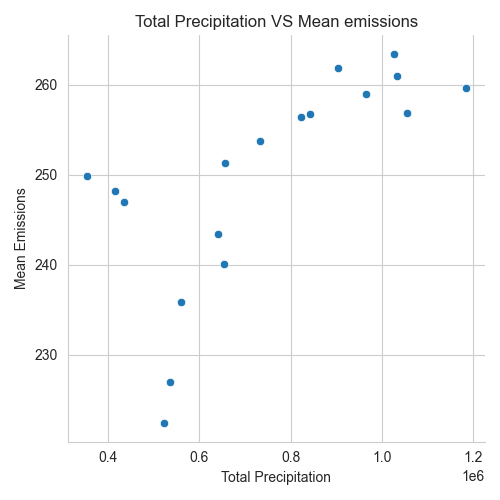
\includegraphics[width=1\columnwidth]{plots/Total Precipitation VS Mean emissions.png}
            \caption{Zależność pomiędzy opadami i ilością emisji}
            \label{fig:precipitation_vs_emissions}
        \end{figure}

    \subsection*{Wyszukiwanie zależności}
        Na podstawie statystyk trudno wywnioskować zależności pomiędzy średnią temperaturą, populacją a danymi pogodowymi, jednak to nie oznacza, że żadnej zależności nie ma. Na niektórych wykresach można zobaczyć podobeństwo zależności.
        
        Jednak możemy zobaczyć bardzo dobrą zależność pomiędzy pojemnością silnika, ilością cylindrów, wykorzystanym typem paliwa a wskaźnikiem zużycia paliwa. Także, na wykresie \ref{fig:fuel_cons_vs_emissions} można zobaczyć interesującą zależność od typu wykorzystanego paliwa z którego można wywnioskować, że diesel robi najwięcej emisji przy takim samym zużyciu, benzyna premialna ma największy wskaźnik zużycia/emisji (z tego powodu że benzyna premialna jest wykorzystana w samochodach premium klasy, np. Porsche, Ferrari itd., które mają duże silniki i wysoką moc) oraz to, że etanol jest najbardziej ekologicznym paliwem, ponieważ przy dowolnym zużyciu paliwa zawsze produkuje znacznie mniej emisji niż inne paliwa.

\section*{Modele przewidywające}
    \subsection*{Wstępne przetwarzanie danych}
        Dlatego aby stworzyć model, który przewidzi zużycie paliwa najpierw potrzebujemy dodać wszystkie dane do jednego zbioru danych. Głównym zbiorem danych w danym przypadku to zbiór samochodów wraz z ich zużyciem paliwa. Dane samochodu łączone są z danymi o średniej temperaturze, populacji i sprzedanych samochodach na podstawie roku produkcji samochodu, tzn. zestaw danych podstawowych dla każdego unikalnego roku produkcji będzie miał tą samą wartość, która odpowiada jego wartości i rokowi w oryginalnym zbiorze.
        
        Dla trenowania został wybrany okres od 2000 do 2017 roku, ponieważ w tym scenariuszu mamy wszystkie potrzebne dane.

        Następnie, dla trenowania były wyrzucone niepotrzebne dane, które nie mają wpływu na zużycie paliwa: \textit{Marka, Model, Typ Samochodu, Transmisja}. Także musimy usunąć inne wskaźniki zużycia paliwa i emisji: \textit{HWY (L/100 km), COMB (L/100 km), COMB (mpg), Emisje}, ponieważ one są wyliczane na podstawie zużycia paliwa.
        
        Ostatnim krokiem jest zmiana wartości typów paliwa. Ponieważ modele mogą trenować się tylko na podsawie danych numerycznych, typy paliwa są zmieniane na odpowiednie liczby:\\
        \begin{itemize}
            \item 1 - Benzyna zwykłą
            \item 2 - Benzyna premialna
            \item 3 - Diesel
            \item 4 - Ethanol
            \item 5 - Naturalny gaz
         \end{itemize}
        
    \subsection*{Tworzenie modeli przewidywających}
        Dla tworzenia zbiorów trenujących i testowych była wykorzystana metoda \textit{train\_test\_split} z biblioteki scikit-learn. Następnie za pomocą tych zbiorów były trenowane pięć różnych modeli: \textbf{Regresja liniowa}, \textbf{Uogólniony model liniowy (GLM)}, \textbf{XGBoost}, \textbf{Maszyna wektorów nośnych (Scaled SVM)}, wykorzystująca dodatkową bibliotekę doprowodzająca dane do jednej skali w celu uzyskania dobrych wynkików uczenia się, i \textbf{Metoda lasu losowego (Random Forest)}.

        Po trenowaniu i przewidywaniu możliwych wartości spalania paliwa, były otrzymane rezultaty pokazane w tabeli \ref{tab:models_results}:

        \begin{table}[h]
        \centering
        \caption{Porównanie wydajności modeli}
        \label{tab:models_results}
        \begin{tabular}{lcccc}
        \toprule
        Model                  & MAE      & MSE      & RMSE     & \(R^2\)\\
        \midrule
        Regresja liniowa       & 1.303577 & 3.156626 & 1.776690 & 0.754250\\
        GLM                    & 1.374618 & 3.376737 & 1.837590 & 0.737114\\
        \textbf{XGBoost}                & \textbf{0.887038} & \textbf{1.519095} & \textbf{1.232516} & \textbf{0.881735}\\
        Scaled SVM             & 1.070279 & 2.328741 & 1.526021 & 0.818702\\
        Random forest          & 0.894831 & 1.556078 & 1.247428 & 0.878856\\
        \bottomrule
        \end{tabular}
        \addtabletext{MAE - Średni błąd bezwzględny\\
                      MSE - Średni błąd kwadratowy\\
                      RMSE - Pierwiastek średniokwadratowy błędu\\
                      }
        \end{table}

        \begin{figure}[H]
            \centering
            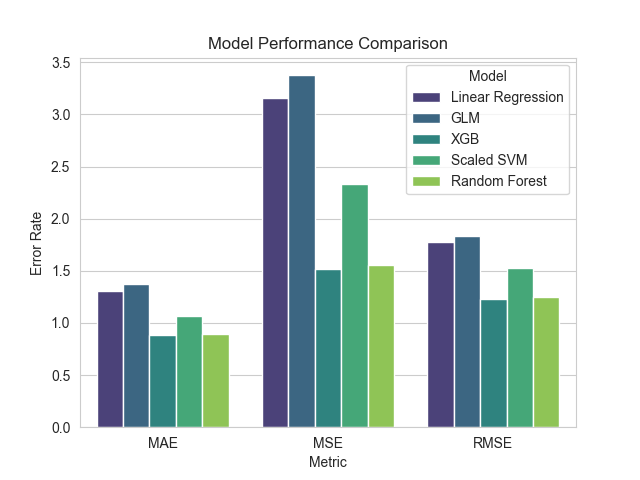
\includegraphics[width=1\columnwidth]{plots/Model Performance Comparison.png}
            \caption{Porównanie wydajności modeli}
            \label{fig:perfomance_comp}
        \end{figure}

        \begin{figure}[H]
            \centering
            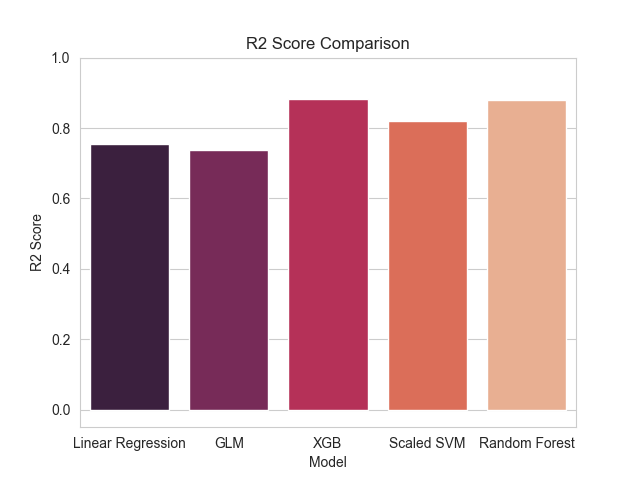
\includegraphics[width=1\columnwidth]{plots/R2 Score Comparison.png}
            \caption{Porównanie wyników \(R^2\)}
            \label{fig:perfomance_comp_r2}
        \end{figure}

        Współczynnik \(R^2\) reprezentuje procentową zmienność zmiennej zależnej, która jest wyjaśniona przez niezależne zmienne w modelu. Wartość \(R^2\) jest zazwyczaj pomiędzy 0 a 1, gdzie 1 oznacza idealne dopasowanie, a wartość bliższa 0 oznacza, że model słabo wyjaśnia dane. Wysoki współczynnik \(R^2\) wskazuje na to, że model dobrze pasuje do obserwowanych danych.

        Na podstawie wyników z tabeli \ref{tab:models_results} i wykresów \ref{fig:perfomance_comp} oraz \ref{fig:perfomance_comp_r2}, można wywnioskować, że w naszym przypadku najlepsze przewidywanie danych osiąga model \textbf{XGBoost}.

        Wykres \ref{fig:models_deviation} pokazuje odchylenie przewidzianych wartości od wartości prawdziwych.

        \begin{figure}[H]
            \centering
            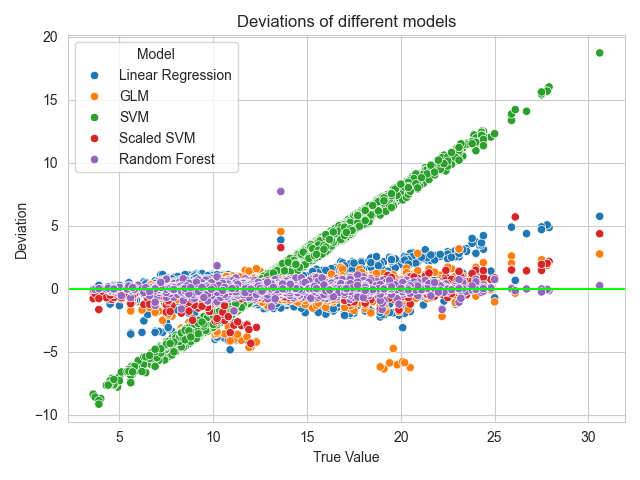
\includegraphics[width=1\columnwidth]{plots/Deviations of different models.png}
            \caption{Odchylenia różnych modeli}
            \label{fig:models_deviation}
        \end{figure}

\section*{Wnioski}
    Analiza i modelowanie zużycia paliwa w samochodach na podstawie zgromadzonych danych z różnych źródeł dostarczyło istotnych wniosków. Przeprowadzone badania wykazały, że model \textbf{XGBoost} był najbardziej efektywny w przewidywaniu zużycia paliwa, co zostało potwierdzone najwyższym wynikiem współczynnika \(R^2\) i błędów MAE, MSE i RMSE. Wysoka wartość współczynnika \(R^2\) wskazuje na dobrą zdolność modelu do wyjaśniania zmienności danych oraz możliwość stosowania tego modelu w przyszłości dla oszacowania przybliżonego zużycia paliwa bez potrzeby na dodatkowe badania. Dodatkowo, integracja danych z różnych źródeł, takich jak warunki pogodowe, demografia i sprzedaż samochodów, pozwoliła na stworzenie bardziej złożonego i dokładnego modelu.

%----------------------------------------------------------

\printbibliography[title={Źródła}]

%----------------------------------------------------------

\end{document}